\documentclass{sig-alt-release2}
\usepackage{url}
\usepackage{color}
\usepackage{graphics,graphicx}

\usepackage{epsfig}
\usepackage{epstopdf}
\usepackage{amsfonts}

\usepackage{colortbl}
\usepackage{multirow}
\usepackage{booktabs}
\usepackage{ifthen}  

\begin{document}
\newcommand{\todo}[1]{\textcolor{red}{#1}}
\def\newblock{\hskip .11em plus .33em minus .07em}

\conferenceinfo{DIM3} {2012, Glasgow, UK} 
\CopyrightYear{2012}
\clubpenalty = 10000
\widowpenalty = 10000

\title{Popcorn \-- the Film Search Engine and Reviewing Application}

\numberofauthors{5}
\author{
\alignauthor
Jessica Bell, Marco Sarconi, Hristo Georgiev, Xun Zhang, David McBrierty\\
	   \affaddr{Group D}
      \affaddr{Dim3}
      \affaddr{}
             \email{\{0807335b, 0806240h, 1003619g, 1105765z, 0502862m\}@student.glasgow.ac.uk }
}
\maketitle

\begin{abstract}
Popcorn is a multimedia search mash-up. It is designed to provide a simple interface with reliance on Django and PuppyIR framework, letting users search for films and write reviews for them.

\end{abstract}

\section{Aim of Application}
Popcorn is a search engine based web application for films, that provides results with collated information on the selected film and the ability for registered users to review the film. This uses the PuppyIR Framework \cite{puppyir} to bring information together from many other web services, such as IMDb \cite{imdb} for the film details and YouTube \cite{youtube} for trailers. 
 
The goal of the design is to provide a useful and intuitive application, that satisfies the user's query about a film, and allows them to easily give their opinion through the review feature. 
 
The project is constrained by the small amount of time to complete the application with a relatively small team to work on it. Although many ideas have been formed about the functionality of the application, it would not be possible to implement them all in the time available. Also the project is constrained in terms of the language and tools used to create it, as the team is inexperienced in building web applications. The application will be implemented using the Django framework, as the team has had most experience with it, and as it is requested by the course lecturer. 
 
 
The must-have requirements are displayed in the user matrix (Table \ref{usermatrix}) below, with the columns indicating the functionality available to the two user groups of logged in (registered) and not logged in (guest) users .

\begin{table}
\begin{tabular}{| l | c | c |}
\hline
& Guest & Registered \\
\hline
Search films by title, actor, genre, keyword & \checkmark & \checkmark \\
\hline
View recent user past searches & \checkmark & \checkmark \\
\hline
See overall most viewed films & \checkmark & \checkmark \\
\hline
Produce random film result & \checkmark & \checkmark \\
\hline
View specific film information & \checkmark & \checkmark \\
\hline
Rate film search results & \checkmark & \checkmark \\
\hline
Look at other user reviews & \checkmark & \checkmark \\
\hline
Review films & & \checkmark \\
\hline
\end{tabular}
\caption{User needs matrix}
\label{usermatrix}
\end{table}

If time allows, the would-like requirements are for users to be able to:
\begin{itemize}
\item find out where they can buy the film or see in the cinema
\item rate or comment on other users' reviews
\item view films recommended for them by their past interactions with the application.
\end{itemize}
However the must-have requirements should be sufficient for the time the team has to develop the application.


The scope of the application is wide enough for the basic functionality of providing film information and reviews, but could be extended to provide more use with recommendations. The design goals may be somewhat ambitious considering the constraints, but with good team work should be manageable. The application is fairly complex, as it will be using several different APIs to get the search result information, requires several databases to be managed, and will implement a log in feature. The distribution of the application is most appropriate across the web, as it is one of the primary sources of information that people go to when they have a query, and films are increasingly connected with the web as television and films become more widely distributed over it.


\section{Client Interface} %%%%%proper walkthrough
The wireframes and descriptions of the user interface are included in the appendix (see Figures 1, 2 and 3). Two user personas can be imagined in the different ways to use the site. The first would be a person looking for a film to watch, but unsure of a specific film title. Their usage of the site would be for example entering a preferred genre such as sci-fi, looking through the results given, and selecting a film that looks interesting, to view more information about the film and watch the trailer. They watch the film and if they enjoy it, select the 'like' rating on the film information page. The second would be a person that is interested in film, or potentially a film student,  and likes to give their opinion on films they have watched. They would log in, search the site for a specific film title, and after selecting it on the results page, read other reviews and create their own. 
 
There will be several dynamic components included on the user interface, such as the quick rating buttons, buttons to remove results from the past searches box, liked films box and from the results list, and the moveable and resizeable information boxes on the film information pages. This will help the user to arrange the information on the page as suits them best. The PuppyIR framework and other applications built from it such as MaSe, support this rearrangement of components in the client browser, so this can be used to implement this feature in the application. The other dynamic components can be supported using XML and JQuery. 
 
The user interface should be visually appealing, intuitive and simple enough to use, so that the user can complete their required task without difficulty. On the client side, the application will be implemented using HTML and CSS will be used to display the information, which is also beneficial in providing a separation of concerns between the structure and the style of the application.


\section{Application Architecture}
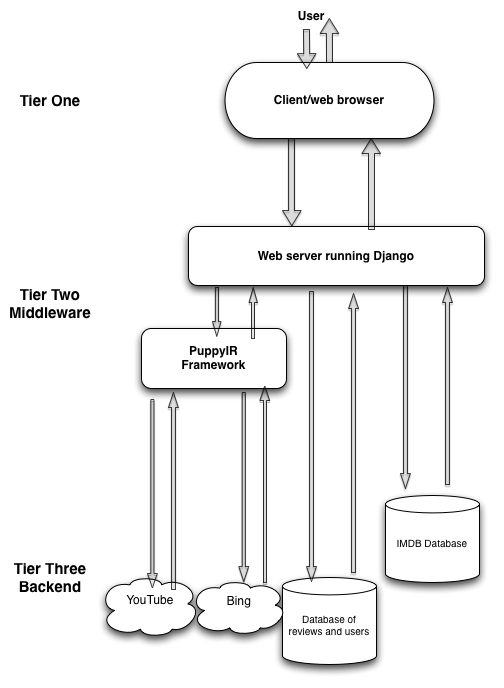
\includegraphics[scale=0.4]{tier.png}
Popcorn will utilise the puppyIR framework in order to allow basic search functionality and to gather content from different search providers. 
 
Tier 1: The client 
 
The client - a web browser - displays the front end of the web service to the user, allowing them to view and interact with the service without knowledge of the middleware and backend. The browser visualises the information in a user friendly form via HTML and CSS. At this stage no specific style sheet will be created for mobile web browsers and as such the user experience may be impaired on a mobile device. 
 
Tier 2: Server 
 
The Server Tier receives queries from the client and takes required action to search relevant search services to service the user. User preferences are fetched from the Database in Tier 3. These preferences include which services to use in the search. Results from the different backend services are prepared by this tier for presentation by the client. 
 
This tier is represented by a server running Django, it handles all the requests from the client forwarding them to the relevant backend service or to the PuppyIR framework which then carries out a web search and returns the results to the Django server. The server then deals with the various responses, processing them for display to the client. 
 
Tier 3: Database and APIs 
 
Our own sqlite database stores Popcorn's users and their credentials as well as reviews written by the users. It also stores data about each film- a unique ID corresponding to the IMDb's movieID, the number of times this movie has been selected, a rating and the number of times this movie has been 'liked'. 
 
film data is gathered via the IMDB using IMDbPy - a python service for searching the 'IMDb' database. Other information about the film is collected through search services such as 'Bing' and 'YouTube' which interface with PuppyIR. 
 
 
DATA MODEL

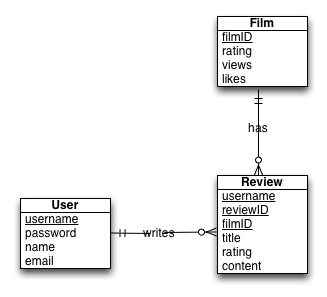
\includegraphics[scale=0.6]{erdiagram.png}
 
The data model contains three tables: user, film and review. 
 
User: Used to store log-in credentials of users and email address for possible future enhancements such as a weekly e-mail recommended films. Although it is not necessary to login to use the service, the user must be a member of the site in order to write a reviews. This decision was taken to help minimise spam or 'trolling' of the review feature. We felt users who were keen to write reviews would not mind the minor inconvenience of setting up an account. Moreover, additional benefits like, for instance, member ratings are available. 
 
Film: This table stores the number of likes a film has received and the number times it has been viewed and a rating which is calculated by the formula (likes/numRatings) * 10. It also stores a unique filmID which corresponds to the movieID from IMDb's film database. This means that we do not need to store all film data such as actors, genres, plot listings etc. Instead, we can link our film statistics (i.e. rating) with the data pulled from IMDb. 
 
Review: This stores review data entered by the users. Each review is linked to a user (via userID) and to a film (by filmID), which all together form the table's primary key. The review contains the main body, a title, numerical rating for the film, and statistics about the number of users (both anonymous and registered) who have found it useful. 
Back end services 
 
 
PuppyIR 
 
PuppyIR is a search framework, funded by the European Union, which provides tools to allow creation of search engines for children. \cite{puppyir}
 
Popcorn will utilize PuppyIR to provide a simple means of searching YouTube, Bing and Yahoo for movie information and trailers. It will also provide us added functionality such as query logging,and query suggestions which will cut our development time. PuppyIR is implemented in python and interfaces with django as such we feel it meets the needs of this project. 
 
IMDb 
 
As IMDb does not provide its own API we have decided to utilise IMDbPy.  IMDbPY is a Python package used to retrieve and manage the data of the IMDb movie database about movies, people, characters and companies. \cite{imdbpy}
It is capable of returning the results of an IMDb search in XML format. 
 
 
Separation Of Concerns 
 
Separation of concerns is ensured by the system design, in utilising an n-tier architecture we have ensured that each part of the system has its own responsibilities and that changes to one tier should not necessarily require changes to be made to the others. By using both HTML and CSS we can maintain seperation of concerns in that the results or data displayed by HTML need not be altered if we wish to change the style via CSS, to provide a mobile layout for example. 
 
WEB FRAMEWORK 
 
Although using a web application framework is not necessary for a project of this scale it allows for a rapid development as the framework provides functionality which would otherwise have to be implemented.  Having decided to utilise a web framework, we then  selected django because it is modern and lightweight while still providing ample functionality. A further advantage of django is that programming is done in python with which the team are familiar. This should save development time. Although we could have selected an alternative framework such as Java Struts, we felt that django was the better choice and more suited to this projects needs. 
 
Using a web framework has many advantages, such as providing a structure and basis for the application and helping to enforce separation of concerns: the model view controller pattern . They also allow for a faster development time by implementing their own session and cookie management, providing database connectivity as well as admin services. 
 
Unfortunately web frameworks do come with some disadvantages, in that they limit choice and flexibility, and your service must conform to a structure laid out by the framework.

\section{Message Parsing}
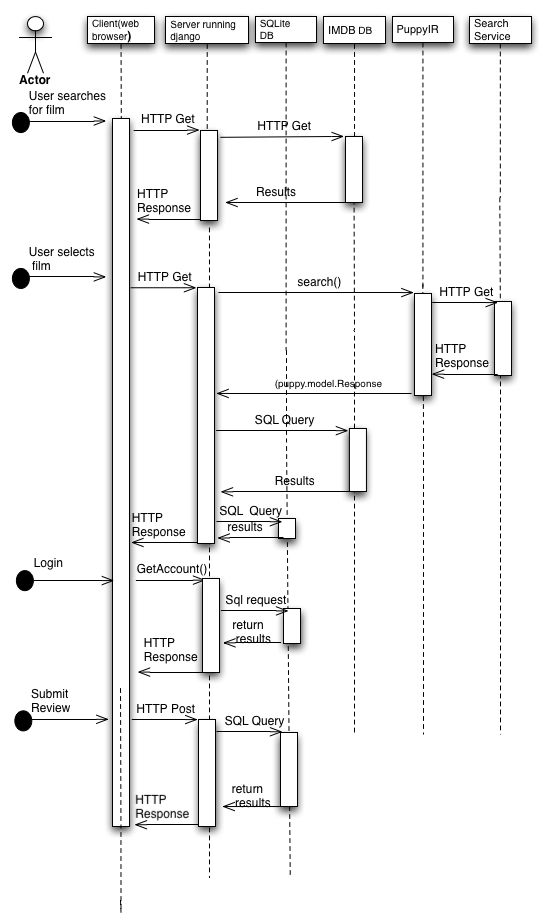
\includegraphics[scale=0.4]{seqdiagram.png}

FORMAT OF THE MESSAGES 

HTTP GET \& RESPONSE
The user could search for films and select films without logging in to the system. Any public user could make a http request to the server. And then the server returns the result by a http response. For instance, the server would pass the request to IMDB, also using a http request. The advantage of this format is that this is the  de-facto standard which is supported by all the frameworks including Django. 

XML 
The IMDB interface returns any result using XML. We use XML because it is supported by all the search engine  APIs and Django supports XML directly. The disadvantage of XML is that it is slower to parse when compared to JSON, with JSON you can parse it using eval() using Javascript. 

SQL Query 
We use SQLite database because it is embedded in the Django framework. We could have use other database like mySQL, Oracle, etc. But we considered that the time for developing this web application is rather limited and we could make good use of Django framework, which is what we have learned from this course. All of the queries are Restful ones, this format was selected as all the search engine APIs are compatible with it so it reduced the overhead associated with using multiple formats.





\section{Design Revision / Feedback}
{\bf For the Implementation Report Only:}
\begin{itemize}
\item	include a summary of the feedback given (or refer to specific comments from the feedback) 
\item	comment on how you have revised the design (if at all) according to the comments received 
\item	how has the feedback helped, and has this process been helpful.
\end{itemize}

\section{Implementation Notes}
{\bf For the Implementation Report Only:}

\begin{itemize}
\item Views - What are the main views that you have implemented and what do they do?
\item URL Mapping Schema - what is your URL mapping and schema?
\item External Services  - what external services does your application include and what handlers did you include?
\item	Functionality Checklist (which functionality is completed)
\item	Known Issues (what kind of works, what kind of errors to do you get)
\item What technologies have been used and are required for the application. Include a list or table of all the technologies, standards, and protocols that will be required.
\end{itemize}

\section{Reflective Summary}
{\bf For the Implementation Report Only:}
\begin{itemize}
\item	What have you learnt through the process of development? 
\item	How did the application of frameworks help or hinder your progress? 
\item	What problems did you encounter? 
\item	What were your major achievements?
\end{itemize}

\section{Summary and Future Work}
 
SUMMARY  
 
This service is currently in development. On completion we hope to offer an interesting, intuitive web service based around finding films to watch and reviewing those films. The main limitations for this project are the very limited timescale and a restriction on available resources. 
 
LIMITATIONS 
 
The project is constrained by the small amount of time to complete the application with a relatively small team to work on it. Although many ideas have been formed about the functionality of the application, it would not be possible to implement them all in the time available. Also the project is constrained in terms of the language and tools used to create it, as the team is inexperienced in building web applications. The application will be implemented using the Django framework and PuppyIR framework, as the team has had most experience with it, and as it is requested by the course lecturer. 
 
PLANS FOR FUTURE DEVELOPMENT
 
Support of user ranks could be implemented. For instance: (special ranks) Site Administrator, Moderator; (ranks based on the number of reviews made) Newbie 0, New user 10, Novice 50, Active user 100, VIP user 500, Legend 1000 etc. 
 
Another feature that could be added to the project is the support of registered users being able to add comments (and 'find them useful', i.e. rate them) to reviews, thus introducing some form of hierarchy. This would give users the ability to criticise a particular review, or agree or disagree partially with it, by being more specific in the corresponding comment. 
 
Also, the film information could be made editable, i.e. maintained in a wiki style by having open discussions about the different sections of a particular set of film data. Thus, any registered (and trusted - this could be implemented by allowing only users meeting particular requirements, e.g. minimum number of reviews made, in addition to a minimum rating - which can be combined with or derived from the rank support feature) user could help improve and keep the site up-to-date. 
 
Additional film information could be added. For instance, where a particular film can be purchased (providing a list of online shopping services). 
 
Functionality that was initially discussed but decided would require too much time, would be to supply personalised film recommendations, possibly as a substitution for the random film feature on the main page. This could be based on a registered users film ratings, past searches and films viewed, or by the user entering certain preferences, and then using some form of algorithm to create a list of films to recommend. There are several methods that could be used to implement this, so research would need to be done to decide on the best way this could be achieved.

\section{Acknowledgements}
Our thanks to the lecturers and demonstrators for their comments and suggestions.

\section*{}
\begin{thebibliography}{9}
\bibitem{puppyir} Glassey R, Polajnar T and Azzopardi L 2011 PuppyIR Unleashed: A Framework for Building Child-Oriented Information Services {\it The Dutch-Belgian Information Retrieval Workshop, Amsterdam, Netherlands}
\bibitem{imdb} IMdB: {\it www.imdb.com}
\bibitem{youtube} YouTube: {\it www.youtube.com}
\bibitem{imdbpy} IMdBPY: {\it http://imdbpy.sourceforge.net/}
\end{thebibliography}

%\bibliographystyle{abbrv}
%\bibliography{sig-proc}

\appendix
\section{Wireframes}
Figure 1\\
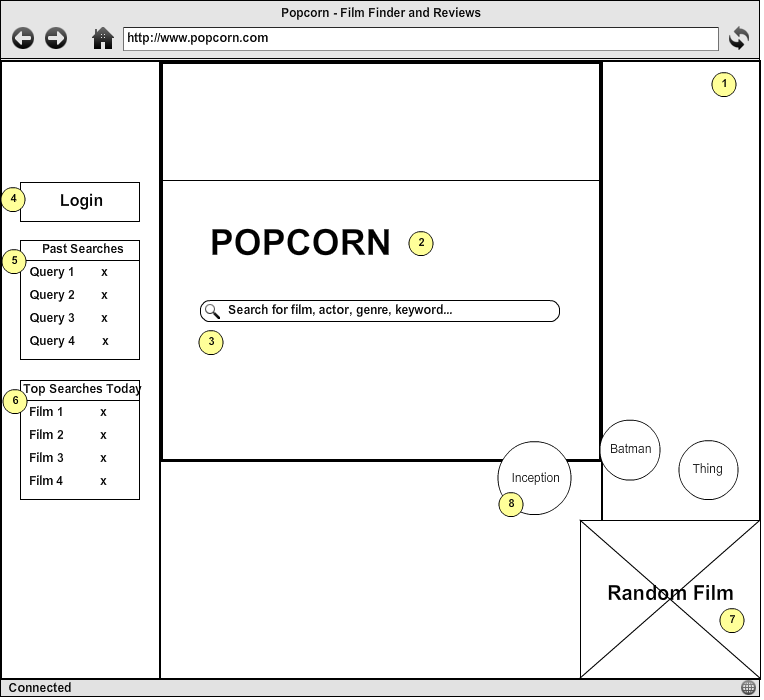
\includegraphics[scale=0.3]{wireframe1.png}
 
1 - Background image of cinema screen \\
2 - Logo \\
3 - Search field, with search instructions when not selected \\
4 - Log in - expands to allow entry of username, password, or registration \\
5 - If users has already searched in current session, the last searches (to a maximum of 5) are shown \\
6 - The most viewed films by all users in the last 24 hours are shown here \\
7 - An image of a popcorn box, that when clicked leads to an information page of a random film \\
8 - Images of popcorn with random film titles on, that lead to the respective film information pages\\


Figure 2\\
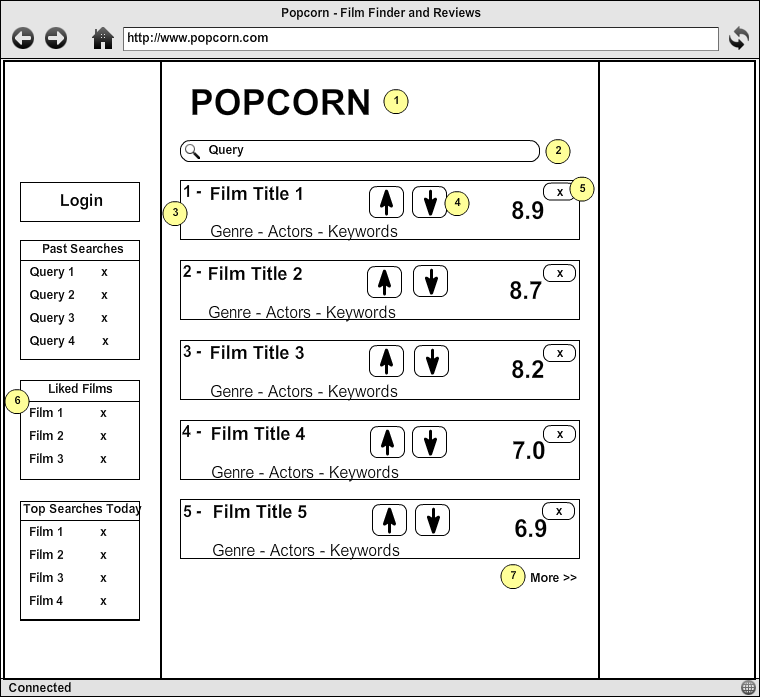
\includegraphics[scale=0.3]{wireframe2.png}
 
1 - Logo, links to main search page \\
2 - Search field, containing current query \\
3 - Film result with summarised information: genre, actors, keywords, rating \\
4 - Quick rating buttons - like or dislike, with liked films showing up in box 6 \\
5 - Remove result button, the result is removed and next result is added to bottom of list - the result is removed only during the current search, and would reappear when searched again \\
6 - Liked films, with x to remove like rating \\
7 - Show next 5 search results\\

Figure 3\\
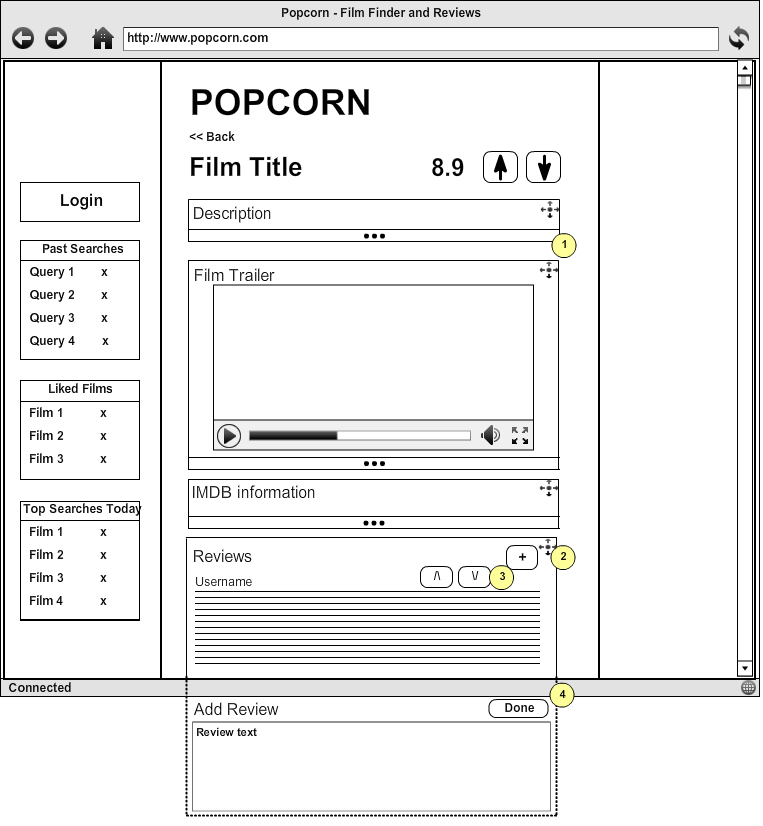
\includegraphics[scale=0.3]{wireframe3.png}
1 - Moveable, resizeable information boxes \\
2 - Reviews with add review entry at bottom of page, and add review button to jump to it \\
3 - Like and dislike quick rating buttons for individual reviews \\
4 - Create review form at bottom of page, after scrolling past all reviews or using the add review entry button at top of reviews to jump to the section\\



\end{document}
